\documentclass{standalone}

\usepackage{tikz}
\usepackage[T1]{fontenc}
\usepackage[tt=false, type1=true]{libertine}
\usepackage[varqu]{zi4}
\usepackage[libertine]{newtxmath}

\usetikzlibrary{shapes, positioning, calc}

\begin{document}

{\scriptsize
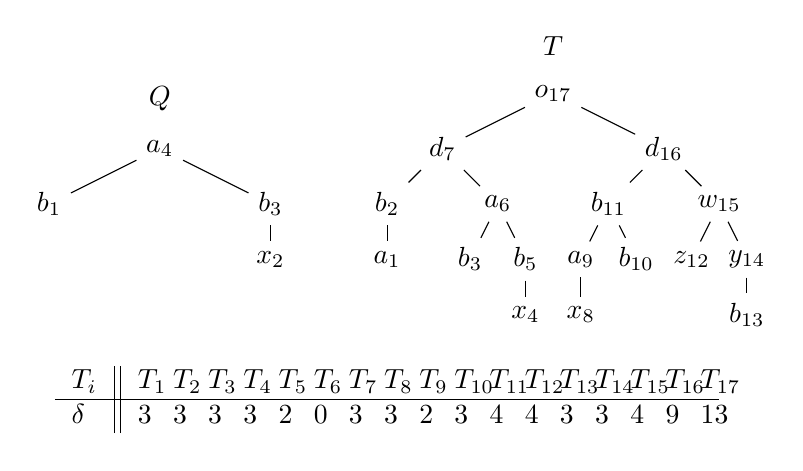
\begin{tikzpicture}[
    % thick,
    level distance=2em,
    level 1/.style={sibling distance=8em},
    level 2/.style={sibling distance=4em},
    level 3/.style={sibling distance=2em}]

  % document
  \node at (0, 0) (t-root) {$o_{17}$}
  child {
    node (d7) {$d_7$}
    child {
      node {$b_2$}
      child { node (a1) {$a_1$} }
    }
    child {
      node {$a_6$}
      child { node {$b_3$} }
      child {
        node {$b_5$}
        child { node {$x_4$} }
      }
    }
  }
  child {
    node (d16) {$d_{16}$}
    child {
      node {$b_{11}$}
      child {
        node {$a_9$}
        child { node {$x_8$} }
      }
      child { node {$b_{10}$} }
    }
    child {
      node {$w_{15}$}
      child { node {$z_{12}$} }
      child {
        node {$y_{14}$}
        child { node {$b_{13}$} }
      }
    }
  };
  \node[above=0.125 of t-root] (t) {$T$};

  % query
  \node[left=3 of d7] (q1-root) {$a_4$}
  child { node (b1) {$b_1$} }
  child {
    node {$b_3$}
    child { node (x2) {$x_2$} }
  };
  \node[above=0.125 of q1-root] (q1) {$Q$};

  \newcommand\cellwidth{0.025cm}
  \node[below=1 of a1] (distances) {
    \begin{tabular}{l||p{\cellwidth}p{\cellwidth}p{\cellwidth}p{\cellwidth}p{\cellwidth}p{\cellwidth}p{\cellwidth}p{\cellwidth}p{\cellwidth}p{\cellwidth}p{\cellwidth}p{\cellwidth}p{\cellwidth}p{\cellwidth}p{\cellwidth}p{\cellwidth}p{\cellwidth}}
      $T_i$ & $T_1$ & $T_2$ & $T_3$ & $T_4$ & $T_5$ & $T_6$ & $T_7$ & $T_8$ & $T_9$ & $T_{10}$ & $T_{11}$ & $T_{12}$ & $T_{13}$ & $T_{14}$ & $T_{15}$ & $T_{16}$ & $T_{17}$ \tabularnewline
      \hline
      $\delta$ & $3$ & $3$ & $3$ & $3$ & $2$ & $0$ & $3$ & $3$ & $2$ & $3$ & $4$ & $4$ & $3$ & $3$ & $4$ & $9$ & $13$ \tabularnewline
    \end{tabular}
  };
\end{tikzpicture}
}

\end{document}
